% Editorial rewrite of main.tex. No new experiments or numerical results.
% Build from this directory: tectonic --only-cached main-astra-rewrite.tex
\documentclass[reprint,amsmath,amssymb,aps,pra,floatfix,nofootinbib]{revtex4-2}
\usepackage{graphicx}
\usepackage{booktabs}
\usepackage{array}
\usepackage[colorlinks,linkcolor=blue,citecolor=blue,urlcolor=blue]{hyperref}
\urlstyle{same}
\newcommand{\kB}{k_{\mathrm B}}
\newcommand{\noise}{\eta}
\begin{document}
\raggedbottom
\clubpenalty=10000
\widowpenalty=10000
\displaywidowpenalty=10000
\title{CHILL ZEN: Image generation with noisy in-memory reads and local repair}
\author{M. Alexander Nugent}
\affiliation{Knowm Inc.}
\date{\today}

\begin{abstract}
We present CHILL ZEN, a generative architecture that samples discrete image codes using locally trained in-memory lane banks. A global code is drawn autoregressively and repaired; residual patch codes are then drawn in parallel, followed by one joint repair sweep. The procedure uses 3616 noisy lane reads and 131 sequential generation steps, with no equilibrium sampling phase. In the emulator, pooling reduces device noise, so an adjustable comparator supplies most of the sampling variance. On binarized Fashion-MNIST, the two-level model achieves Fr\'echet Inception Distance (FID) 18.09 after grayscale training and 9.69 after binary training, at selected settings on the tested noise grids. A geometry-based energy model gives 2.0\,nJ per image, including readout and a proposed lane decoder, compared with 15.7\,nJ for the published eight-step Denoising Thermodynamic Model (DTM). A selector-column design that avoids the nominal array's sneak paths is estimated at 1.6\,nJ. These are hardware projections, not measurements. The quality comparison uses verified DTM replication code, but the original DTM scoring procedure remains unverified and the training splits differ. The results support a fixed generation procedure with far fewer random draws; realizing its energy benefit requires a comparator and decoder that meet the stated assumptions.
\end{abstract}
\maketitle

\section{Introduction}
Probabilistic hardware uses physical fluctuations to perform computation \cite{conte2019thermodynamic}. Stochastic magnetic devices have demonstrated optimization and learning \cite{sutton2017intrinsic,borders2019integer,niazi2024training}, and transistor-based samplers have motivated dedicated generative architectures \cite{jelincic2025dtm,freitas2025taming}. Their energy cost depends on both the cost of a random draw and the number of draws needed to produce a useful sample.

The Denoising Thermodynamic Model (DTM) addresses a difficulty of energy-based generation: a model that represents distinct modes well can be slow to mix between them. It reverses a noising process through a sequence of relatively easy sampling problems, following the principle of diffusion models \cite{sohldickstein2015deep,ho2020ddpm}. Its proposed hardware, the Denoising Thermodynamic Computer Architecture (DTCA), implements each stage with a sparse bipartite Boltzmann machine. The eight-step configuration uses about $10^7$ random conditional updates per image \cite{jelincic2025dtm}.

CHILL ZEN represents an image as an additive discrete code, draws that code in a fixed sequence, and applies local repair. It has no equilibrium distribution to reach and no mixing phase. The name expands to Comparator-Heated In-memory Lane Learning with Zero-Ended Noise: noisy reads generate symbols, and nominally noiseless reads repair them. Throughout this paper, \emph{sampling temperature} means read-noise amplitude, not physical device temperature.

The hardware constraint is central to the method. A lane pools selected differential conductance pairs into one score. Pooling reduces device noise, leaving too little randomness for generation at the assumed read voltage. A comparator at each lane therefore serves both as readout and as the main source of sampling noise. The prospective energy benefit comes from reducing sampling work, rather than from making each random draw cheaper than a DTCA update.

We evaluate the architecture on Fashion-MNIST \cite{xiao2017fashion}, test its dependence on comparator noise, and estimate inference energy from its operation counts and a stated geometry. All image results come from an emulator. The lane system, adjustable comparator, and analog decoder have not been demonstrated together in hardware.

\section{Representation and generation}\label{sec:method}
\subsection{An additive image code}
The model uses additive quantization with dropout, building on vector and additive quantization \cite{gray1984vq,jegou2011product,babenko2014additive}. Each of $k$ codebooks contains $S$ atoms. An image code selects one atom $a_j$ from each book. With bias image $b$ and independent masks $r_j\sim\mathrm{Bernoulli}(p)$, the fitting objective is
\begin{align}
\mathbb E_r\left\|x-b-\sum_j r_j a_j\right\|^2
&=\left\|x-b-p\sum_j a_j\right\|^2 \nonumber\\
&\quad+p(1-p)\sum_j\|a_j\|^2.
\label{eq:aq}
\end{align}
Codebooks are fitted on the host by alternating discrete encoding with a joint double-precision ridge solve. Complete and partial codes use the same decoder,
\begin{equation}
\hat x=b+p\sum_{j\in\mathrm{present}}a_j.
\label{eq:decode}
\end{equation}
At $p=1$, Eq.~\eqref{eq:aq} reduces to ordinary additive quantization. Dropout makes partial codes part of the fitting objective, although it does not guarantee that every partial code decodes coherently.

The evaluated model has two levels. The \emph{backbone} is a global code with 128 books of 16 symbols, fitted at $p=0.5$. It uses 512 bits. The \emph{patch code} represents the residual with two 16-symbol books at each of 49 nonoverlapping $4\times4$-pixel positions. It adds 392 bits. Together, the levels contain 226 symbols and 904 bits, excluding the class label. Their decoded images add to form the output.

This places the model alongside generation from discrete representations \cite{vandenoord2017vqvae,chang2022maskgit}. Its distinctive choices are a fixed linear decoder, separate generator and repair banks, and local lane training. The decoder also admits a proposed in-memory implementation whose energy is included below.

\subsection{Lane scores and local learning}\label{sec:lanes}
A stored weight consists of two conductances, $G_a$ and $G_b$. Define their balance and total magnitude as
\begin{equation}
w=\frac{G_a-G_b}{G_a+G_b},\qquad m=G_a+G_b.
\end{equation}
The differential divider reports $V_y=Vw$ at read voltage $V$. A neural lane pools several selected pairs on a shared output node. For selected addresses $\mathcal A$, its normalized score is
\begin{equation}
y=\frac{\sum_{i\in\mathcal A}(G_{a,i}-G_{b,i})}
        {\sum_{i\in\mathcal A}(G_{a,i}+G_{b,i})}
 =\frac{\sum_{i\in\mathcal A}m_iw_i}{\sum_{i\in\mathcal A}m_i}.
\label{eq:pool}
\end{equation}
An address space supplies one selected symbol. The ordered list of selections is the Activation Address Tuple. Each space contributes in proportion to its selected magnitude, so a conditioning variable can have little influence in a large pool. The class label is therefore repeated in six spaces.

Lanes form winner-take-all groups, with one lane for each possible output symbol. Training uses the kT-RAM local instruction rules \cite{knowm2026blog,knowm2026emulator}. Forward feedback adds magnitude and reverse feedback removes it. The supervised rule reads all lanes, reinforces the target, and pairs forward and reverse operations. A hard rule also penalizes an incorrectly active lane; a soft rule omits that additional penalty. Soft banks generate symbols, while hard banks repair corrupted codes. Appendix~\ref{app:instructions} gives the instruction details.

Magnitude affects adaptation: the same conductance increment changes a large-magnitude pair less than a small one. Under forward-only increments, the two conductances can be interpreted as Beta pseudo-counts. Reverse feedback breaks cumulative counting, so this analogy does not establish a Bayesian posterior or a $1/n$ learning schedule for the deployed rule.

\subsection{A fixed sequence of draws and repairs}\label{sec:sequence}
Let $y_{j,s}(c)$ be the score for symbol $s$ in book $j$ under context $c$. A draw selects
\begin{equation}
z_j=\arg\max_s\{y_{j,s}(c)+\epsilon_{j,s}\},
\quad \epsilon_{j,s}\sim\mathcal N(0,\sigma_{j,s}^2).
\label{eq:draw}
\end{equation}
Noise is independent across lanes in the emulator. This defines a conditional choice distribution; the learning rule does not calibrate it to the data conditional.

Generation proceeds in five stages:
\begin{enumerate}
\item Hold the class label in its six address spaces.
\item Draw the 128 backbone symbols autoregressively with generator bank G1, then apply one parallel repair sweep with bank R1.
\item Draw all 98 patch symbols in parallel with generator bank G2, conditioned on the repaired backbone.
\item Apply one parallel joint repair sweep to all 226 symbols. This can change both backbone and patch symbols using the same pre-sweep state.
\item Decode the two levels with Eq.~\eqref{eq:decode} and add their images.
\end{enumerate}
The generator reads are \emph{hot}: they include device and comparator noise. The repair reads are \emph{cold}: the reported generation uses noiseless decisions. A separate control tests a finite cold-noise floor (Sec.~\ref{sec:noise}). Hot reads use $V=10$\,mV. The energy model assigns $V=50$\,mV to cold reads.

The procedure requires 128 sequential backbone draws and three parallel stages, or 131 generation steps. It uses 2048 hot backbone lane reads and 1568 hot patch lane reads, for 3616 noisy reads in total. The proposed lane decoder adds one parallel step. The emulator instead decodes and renders in host floating point.

The joint repair runs once because additional sweeps degrade the reported metrics. Across eight cold sweeps, the critic score falls from 0.9007 to 0.813, diversity from 0.549 to 0.443, and tone spread from 1.59 to 1.41. Real encoded inputs also drift under repeated repair. The second sweep still changes about 82 of 226 symbols per image, so one sweep is not convergence. Warmer repeated sweeps do not preserve diversity, and using the draw's noise level makes repair ineffective. These controls support a single correction step rather than an iterative sampler.

\section{Training and image quality}\label{sec:results}
\subsection{Setup and evaluation}
We use a seed-0 permutation of all 70\,000 Fashion-MNIST images, with 68\,000 for fitting and 2000 for validation. Generator banks train on Bernoulli-masked codes with labels retained. Repair banks train on codes corrupted by marginal sampling and generator fills; the joint bank uses corrupted two-level states. Repair-training fills use $V=10$\,mV and comparator noise $v_n=5$\,mV. The binary models retain this recipe.

Bank training uses local instructions without gradients. Codebook fitting and image evaluation run on the host. The frozen critic is a pixel classifier, $784\to256\to\mathrm{ReLU}\to10$, trained with Adam. Every bank is probed each epoch on the validation partition, and the best snapshot is retained. This partition also informed noise settings. The results therefore describe selected models, not performance on an untouched test set. Generation seeds measure sampling variation for one fitted set of banks; they do not measure training or selection uncertainty.

Four grayscale metrics describe the output. \emph{Critic} is class-averaged agreement with the requested label. \emph{Diversity} is the fraction of corresponding pixels that differ by more than $1/16$ between same-class image pairs, averaged across classes. \emph{Tone} is the class-averaged standard deviation of per-image mean foreground intensity, expressed in sixteenths. Foreground pixels have intensity at least $1/16$. \emph{Contrast ratio} is foreground pixel standard deviation divided by its real-image value; the stated alarm threshold is 1.10. FID is evaluated separately on binarized images (Sec.~\ref{sec:fid}).

\subsection{The two-level result}
Table~\ref{tab:quality} reports the model at $v_n/V=0.20$, the best tested setting for the grayscale critic. The reconstruction control supplies a real backbone code directly to G2, bypassing G1 and R1, then runs the patch draw and joint repair. It tests these downstream stages together; it does not isolate one source of error.

\begin{table}[tbp]
\caption{Grayscale results at $v_n/V=0.20$. Generated rows are means over three seeds, each with 1000 images. Parentheses give the seed range (maximum minus minimum), not a confidence interval. Real references are the first 100 validation images per class.}
\label{tab:quality}
\begin{ruledtabular}
\footnotesize
\begin{tabular}{lcccc}
Input & Critic & Diversity & Tone & Contrast\\
\colrule
Real & 0.8860 & 0.4866 & 2.362 & 1.00\\
Real backbone & 0.8963 & 0.5184 & 2.004 & 1.13\\
 & (0.0110) & (0.0015) & &\\
Label only & 0.9007 & 0.5487 & 1.590 & 1.14\\
 & (0.0310) & (0.0052) & &\\
\end{tabular}
\end{ruledtabular}
\end{table}

\begin{figure*}[tp]
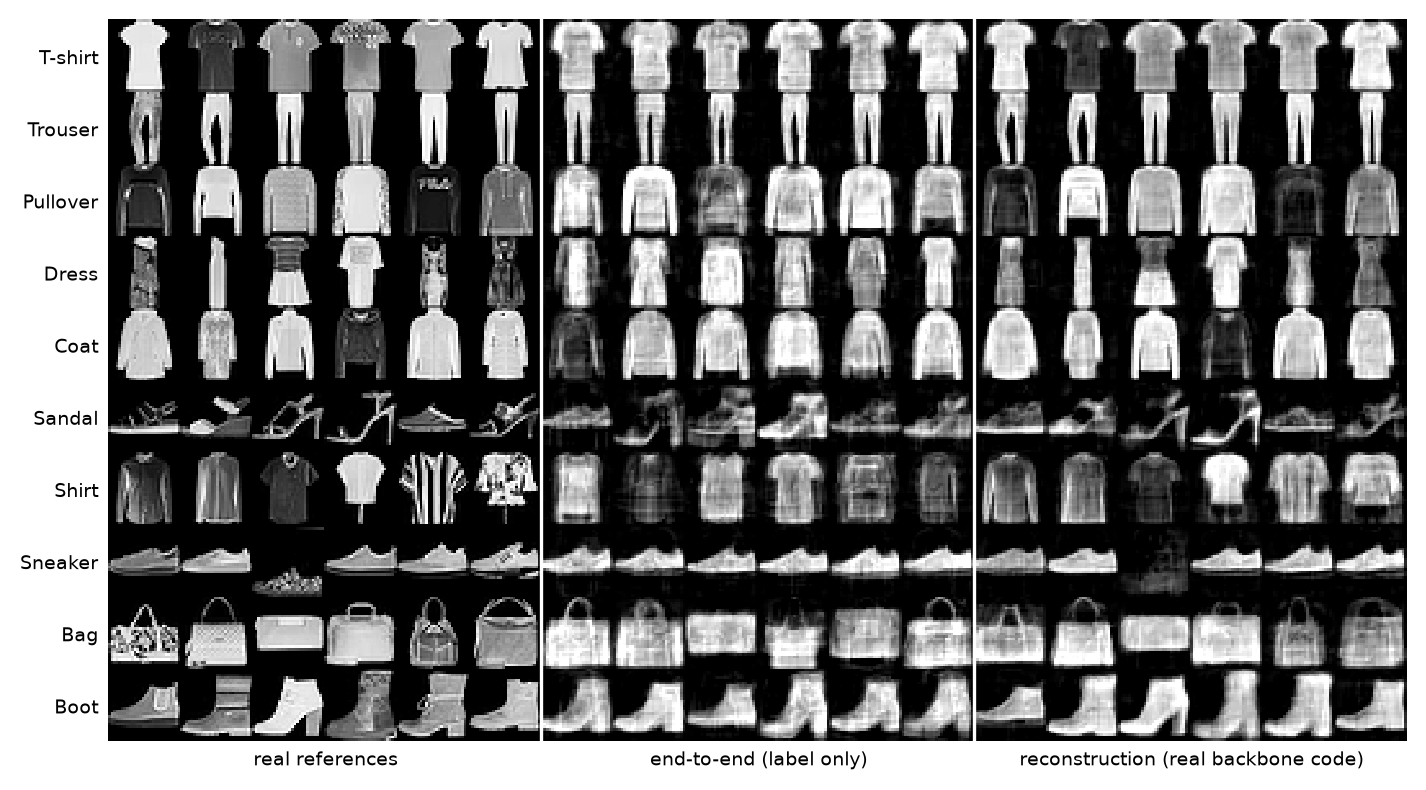
\includegraphics[width=\textwidth]{figures/fig-samples.png}
\caption{Real images (left), generation from labels (center), and the real-backbone reconstruction control (right). Each block shows the first six samples per class from reporting seed 960, without sample selection. Both generated blocks use $V=10$\,mV and $v_n=2$\,mV for hot reads.}
\label{fig:samples}
\end{figure*}

The generated and reconstruction images have critic scores close to the real reference. This establishes label agreement, not equivalent image quality: a classifier can favor class prototypes. Generated tone spread is lower than real, while contrast exceeds the alarm threshold. Figure~\ref{fig:samples} shows the corresponding samples.

An audit of 5120 grayscale draws found distinct backbone and joint codes and no exact training-image copies. Nearest-training-image $L_2$ distances were slightly larger for generated images than for validation images: first percentile 1.86 versus 1.47, and median 3.70 versus 3.43. These checks found no exact-copy signature, but do not exclude all forms of memorization.

\subsection{Representation controls}
The codec studies motivated a global backbone with residual patches. At 512 bits, the global code's lowest relative mean squared reconstruction error is 0.0500 at $p=0.75$. The deployed $p=0.5$ code has higher error, 0.0612, but stronger cross-address coherence in the recorded design studies. Adding residual patches reduces error to 0.0382 (Fig.~\ref{fig:codec}).

Earlier backbone studies increased the critic score from 0.813 to 0.834 when the number of 16-symbol books rose from 64 to 128. A $64\times32$ configuration scored 0.7875, but it also used fewer bits than $128\times16$; this does not isolate alphabet size. These development studies support the chosen representation. They are distinct from the final comparator-setting results reported here.

Reconstruction scores are useful controls, but they do not bound generation scores. In particular, FID compares feature distributions and cannot be separated into additive codec and generator errors. Neither the grayscale reconstruction control nor a backbone-only reconstruction locates all remaining tone and contrast errors.

\begin{figure}[tbp]
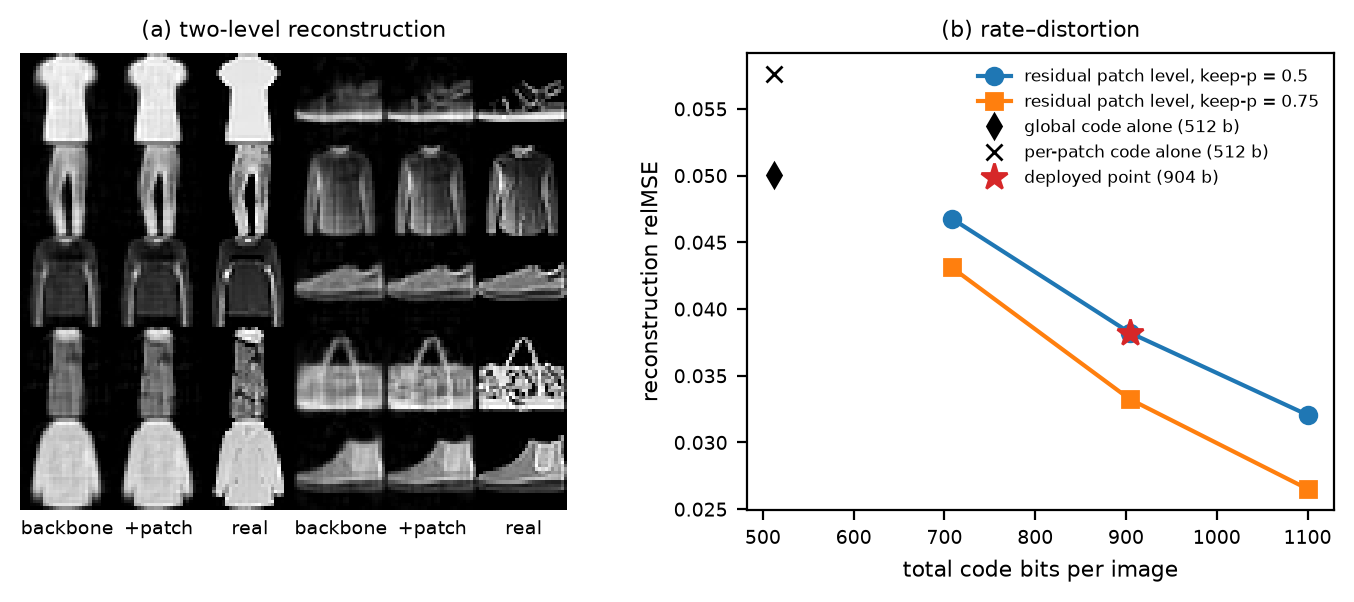
\includegraphics[width=\columnwidth]{figures/fig-codec.png}
\caption{Recorded codec study. (a) Backbone reconstruction, backbone plus residual patches, and the original image. (b) Reconstruction error versus code size. The deployed 904-bit two-level code reaches relative mean squared error 0.0382.}
\label{fig:codec}
\end{figure}

\section{Comparator noise controls sampling}\label{sec:noise}
\subsection{Device noise and pooling}
The modeled read variance contains thermal, flicker, and comparator terms:
\begin{equation}
\sigma_y^2=\sigma_{\mathrm{th}}^2+\sigma_{\mathrm{fl}}^2+
\left(\frac{v_n}{V}\right)^2.
\label{eq:noise}
\end{equation}
Here $v_n$ is the comparator's input-referred rms noise. At fixed pulse width, the device terms scale approximately as
\begin{equation}
\sigma_{\mathrm{th}}\propto\frac{\sqrt{\kB T}}{V\sqrt m},
\qquad
\sigma_{\mathrm{fl}}\propto\frac{1-w^2}{\sqrt m},
\end{equation}
where $T$ is physical temperature. With settling-limited timing, $t=5C_{\mathrm{node}}/G_\Sigma$, where $G_\Sigma$ is pooled conductance, the conductance dependence cancels from the thermal term. A sampled output node has
\begin{equation}
\sigma_{\mathrm{th}}^2\simeq\frac{\kB T}{C_{\mathrm{node}}V^2}.
\label{eq:ktc}
\end{equation}
Pooling increases wiring capacitance and reduces this noise floor. The emulator uses a pulse of $\max(2\,\mathrm{ns},5RC)$; the energy model uses the settling-limited expression.

At the 10\,mV hot-read voltage, the emulator gives device noise of about 0.02--0.04 in normalized score units. Its thermal calculation uses a fixed 100\,fF node. The geometry model instead gives about 12\,fF on the first backbone read, including comparator input capacitance, and 161--278\,fF for the larger pools. That makes the first read noisier, about 0.07, while later reads remain near the emulated range (Fig.~\ref{fig:noise}).

This noise is too small for the reported generation settings. Obtaining the required noise from the output node alone would require a read voltage near 1\,mV, below the assumed 10\,mV sense floor. Device-noise sampling has been used in other memristor systems \cite{dalgaty2021insitu,cai2020hopfield}; here, pooling makes an additional noise source necessary.

\subsection{Noise settings in the emulator}
Write $\noise=v_n/V$ for normalized comparator noise. The emulator provides an 8-bit setting,
\begin{equation}
v_n=100\,\mu\mathrm V+\mathrm{code}\times20\,\mu\mathrm V,
\quad \mathrm{code}\in\{0,\ldots,255\}.
\end{equation}
At 10\,mV, the tested codes 3, 20, 45, 95, 145, and 245 correspond to $\noise=0.016$, 0.05, 0.10, 0.20, 0.30, and 0.50. The device-only control omits comparator noise; it is not register code 0, which retains a finite floor.

The grayscale critic improves over the tested range through $\noise=0.20$. The binary two-level FID is lowest near $\noise=0.20$--0.30 (Fig.~\ref{fig:sweep}); the binary grid was extended after its initial pass. At the grayscale critic setting, the comparator supplies 97--99\% of modeled read variance. Using the smaller first-read capacitance reduces that first-read share to about 90\%.

A voltage control holds $\noise=0.10$ while raising $V$ from 10 to 50\,mV. Device thermal noise falls fivefold, but the grayscale critic changes only from 0.8840 to 0.8837 and binary FID from 10.99 to 10.73. This supports normalized comparator noise as the main sampling control.

\begin{figure}[tbp]
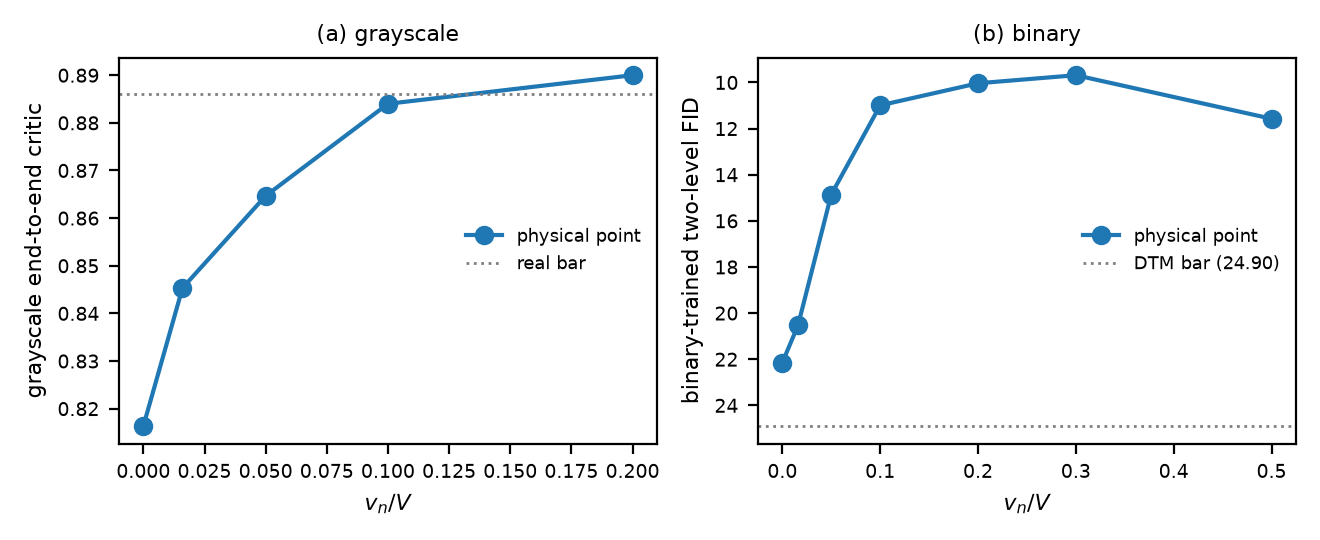
\includegraphics[width=\columnwidth]{figures/fig-comparator-sweep.png}
\caption{Comparator-noise sweeps at $V=10$\,mV. (a) Grayscale critic score. (b) Binary-trained two-level FID under the replication protocol. The horizontal DTM line is its published score, not a rerun. The sweep and Table~\ref{tab:quality} use different generation seeds.}
\label{fig:sweep}
\end{figure}

\subsection{Cold reads and circuit requirements}
Physical cold reads cannot be noiseless. At 50\,mV and the register minimum, the combined modeled noise is about 0.003 of the read voltage. Replacing both noiseless repair stages with this floor changes roughly 9 of 128 R1 decisions and 12 of 226 joint decisions per image. Across three seeds of 1000 images, however, the critic remains approximately 0.890 and diversity, tone, and contrast remain similar. Even at roughly ten times the floor, the mean critic is 0.893 with a seed range of 0.024, compared with 0.890 and a range of 0.012 for noiseless repair. This control supports the cold-read approximation for these aggregate grayscale metrics. FID was not reevaluated with the cold floor applied.

The required comparator must control random noise separately from static offset. At a 10\,mV read, offset should remain below about 1\,mV at every operating bias. The desired hot-noise range is about 2--3\,mV rms for the two-level critic and binary-FID settings, while cold reads require much lower noise. Dynamic latches can provide substantial input noise, but also carry mismatch offsets that require trimming \cite{razavi2015strongarm,pelgrom1989matching}. Reduced preamplifier bias or an added input noise source could supply hot noise.

These are design requirements. No comparator has been designed for this system, and its bandwidth, noise range, offset, kickback, and energy have not been demonstrated together. The emulator assumes independent additive noise and omits kickback. Appendix~\ref{app:readout} makes the readout-energy assumptions explicit.

\section{Binarized Fashion-MNIST}\label{sec:fid}
\subsection{Scoring protocol and comparison scope}
The published DTM reports FID \cite{heusel2017fid} on binarized Fashion-MNIST. Its paper does not specify the feature extractor, sample count, threshold, or label-conditioning mode. We use the DTM replication repository \cite{dtmreplication} linked from the released \texttt{thrml} library \cite{extropic2025thrml}. The replication supplies evaluation code and reference statistics; it does not establish the original paper's exact scoring path.

Our scoring uses its unmodified InceptionV3 extractor and Fr\'echet-distance code: 2048-dimensional pool features, bilinear antialiased resizing to $256\times256$, grayscale repeated in three channels and scaled to $[-1,1]$, and a matrix square root for the distance. Images are binarized at 0.1 on the $[0,1]$ scale. Each generated batch contains 5120 images, 512 per class. Reference statistics cover the canonical 60\,000-image training split.

Passing all 60\,000 training images through this path gives FID 0.000039 against the supplied statistics, verifying agreement with the replication pipeline. The canonical test split gives 2.142 at $n=5120$, a finite-sample real-data reference. It is not a held-out test of CHILL ZEN, because most canonical test images are included in our fitting partition. Our 68\,000-image fitting set also differs in size from the DTM's 60\,000-image training set.

The threshold materially affects the result. The same 60\,000 real training images binarized at 0.5 score 29.75 against the 0.1 reference. We therefore retain the replication's threshold throughout. Published DTM scores are quoted as references; they were not rerun through our scoring pipeline.

\subsection{Results and controls}
Table~\ref{tab:fid} reports results at the selected noise levels. Grayscale models generate images that the host thresholds for scoring. Binary models use the same architecture and recipe, fitted to images binarized at 0.1. They receive binary training data, as the DTM does, but the fitting partitions still differ.

\begin{table*}[tp]
\caption{Binarized-image results. Diversity is within-class mean pairwise pixel disagreement, distinct from the grayscale diversity metric. Energies use the nominal geometry and include the proposed lane decoder. Grayscale settings are selected by FID among tested register settings; binary models use $\noise=0.30$, selected on the two-level sweep. DTM values are published results with unverified scoring details.}
\label{tab:fid}
\begin{ruledtabular}
\begin{tabular}{lrrrr}
System & $\noise=v_n/V$ & FID & Diversity & Energy (nJ/image)\\
\colrule
Real fitting images & --- & 1.91 & 0.181 & ---\\
Grayscale backbone reconstruction, 128 books & --- & 14.21 & 0.163 & ---\\
Binary backbone reconstruction, 128 books & --- & 9.57 & 0.167 & ---\\
Binary two-level reconstruction & --- & 2.83 & 0.176 & ---\\
\colrule
Grayscale two-level & 0.10 & 18.09 & 0.156 & 2.0\\
Grayscale one-level, 128 books & 0.05 & 22.11 & 0.152 & 0.75\\
Grayscale one-level, 64 books & 0.05 & 22.62 & 0.143 & 0.25\\
Grayscale one-level, 32 books & 0.016 & 25.76 & 0.120 & 0.099\\
Grayscale one-level, 16 books & 0.10 & 44.15 & 0.116 & 0.049\\
Binary two-level & 0.30 & 9.69 & 0.147 & 2.0\\
Binary one-level, 128 books & 0.30 & 15.46 & 0.130 & 0.75\\
Binary one-level, 64 books & 0.30 & 15.10 & 0.129 & 0.25\\
\colrule
DTM, eight steps \cite{jelincic2025dtm} & --- & 24.90 & --- & 15.7\\
DTM, two steps \cite{jelincic2025dtm} & --- & 32.60 & --- & 3.92\\
\end{tabular}
\end{ruledtabular}
\end{table*}

The two-level model scores 18.09 after grayscale training and 9.69 after binary training. The grayscale critic and FID prefer different noise settings: at the critic setting, $\noise=0.20$, FID is 21.95. Each reported metric must therefore be read with its stated setting. The binary one-level rows use the two-level model's selected noise level; they are not independent noise optima.

The reconstruction references use real codes from the fitting partition. The 14.21 and 9.57 rows decode only the backbone, whereas 2.83 uses the full binary codec. None is a lower bound on generation FID. Grayscale generation has about 86\% of the real reference's binary pixel disagreement; this single statistic does not establish mode coverage.

Three controls further qualify the scores. First, choosing labels uniformly rather than fixing 512 samples per class gives FID 18.27 after grayscale training and 10.10 after binary training. This samples a specified class prior; it does not learn class frequencies. Second, an independent-Bernoulli baseline gives FID 180.5 with class information and 258.1 without it. Third, all 5120 binary two-level draws are distinct and none exactly copies a fitting image. Their median nearest-training-image Hamming distance is 25 bits, versus 23 for the excluded-from-fit reference; that reference itself contains five training-image duplicates. The binary one-level audits also find no exact copies.

These results establish performance under a reproducible protocol. They do not provide a controlled ranking against the published DTM or its other baselines, because scoring details and training data are not fully matched. Noise selection uses the reported metrics, and no baseline trained by gradients on the same code and connectivity was evaluated.

\section{Energy and implementation}\label{sec:energy}
\subsection{Operation counts and estimated energy}
The DTM and CHILL ZEN perform different work per step, so sequential step counts alone cannot compare energy. The eight-step DTM uses $8\times250\times4900\approx10^7$ conditional updates. Its full update is estimated at about 2\,fJ, including a measured 350\,aJ random-bit source plus modeled bias, clock, and communication energy \cite{jelincic2025dtm}. Our nominal readout alone costs 15\,fJ per lane read. CHILL ZEN's proposed advantage therefore depends on needing far fewer operations.

The model counts address delivery, divider reads, and readout through a comparator and buffer. With the proposed decoder, an image requires 10\,064 lane reads and 1\,781\,920 address assertions. Only 3616 reads are hot. Appendix~\ref{app:energy} gives the census, geometry, and equations.

The nominal estimate is 2.0\,nJ per image: approximately 91\% for address delivery, 8\% for readout, and 1\% for divider reads. The published eight-step DTM point is 15.7\,nJ, extracted from its figure, giving a ratio of 7.9. Its text instead gives about 1.6\,nJ per stage, or 12.8\,nJ for eight stages, which reduces the ratio to 6.4. Both are estimates of inference energy, excluding programming and external transfer.

\begin{table}[tbp]
\caption{Two-level energy scenarios. The first five rows vary the nominal crossbar model. The selector column separately removes its sneak paths. All retain assumed readout and decoder costs; the scenarios are not uncertainty bounds.}
\label{tab:energy}
\begin{ruledtabular}
\footnotesize
\begin{tabular}{lc}
Scenario & Energy (nJ/image)\\
\colrule
Nominal $4\times4$ array, 0.8\,V select & 2.0\\
0.5\,V select & 0.88\\
7\,nm-class periphery & 0.82\\
7\,nm-class periphery, 0.5\,V select & 0.42\\
Pessimistic crossbar corner\footnote{$16\times16$ arrays, separate select lines for the two conductance sides, and 1.0\,V select.} & 8.1\\
\colrule
$16\times1$ selector column, adjacent pass gates & 1.6\\
\end{tabular}
\end{ruledtabular}
\end{table}

The sensitivities in Table~\ref{tab:energy} show the importance of select voltage and peripheral capacitance. Binary and grayscale versions have the same estimated energy because their bank dimensions and operation counts are identical.

\subsection{What the hardware estimate assumes}
The nominal array and the emulator do not implement the same read. In a $4\times4$ crossbar with floating unselected lines and equal device conductances, the selected device contributes only $7/16$ of the conductance seen at the node. Its six row and column neighbors contribute about 48\%, and the other nine devices contribute about 8\%. Feedback is likewise distributed. The emulator reads and updates only the selected pair.

A $16\times1$ selector column eliminates these sneak paths. Its estimated energy is 1.6\,nJ with pass gates beside the array, or 0.91\,nJ with gates stacked along the output node. The selector column is the proposed implementation; its two layouts are separate energy scenarios. These estimates preserve the projected advantage in a geometry consistent with isolated selection, but still assume the readout and decoder costs.

The decoder is another unverified component. Storing equal-scale codebook atoms as differential pairs would allow one output lane per pixel to implement the fixed sum. The present emulator uses floating-point decoding; it has not tested atom quantization, lane-read noise, or analog decoding precision. If lane decoding is unavailable, a digital $784\times226$ matrix-vector product adds an estimated 1.8--8.9\,nJ, assuming 10--50\,fJ per 8-bit multiply-accumulate. The DTM requires no decoder for binary Fashion-MNIST because its output spins are the pixels.

The full model contains roughly $2.9\times10^7$ conductance pairs, or $5.7\times10^7$ memristors. Neither die area nor programming energy is bounded. Rails are assumed active only during each read. Circuit timing, correlated noise, kickback, write disturb from unselected devices, and the extrapolation of device flicker noise to short pulses remain implementation questions.

\subsection{Conditional timing}
With a DTCA decorrelation time $\tau_0\approx100$\,ns and two half-sweeps per Gibbs iteration, eight steps of 250 iterations require approximately $2\times8\times250\tau_0=400\,\mu$s. Separate hardware for all eight stages could ideally deliver one image every 50\,$\mu$s after pipeline fill, while retaining that latency.

CHILL ZEN requires 131 generation steps and one proposed decode step. If each complete step fits the 62.5\,ns window assumed for readout energy, latency is about 8\,$\mu$s. That window has not been shown to accommodate address delivery, settling, readout, and commitment. The comparison is a timing scenario, not a measured speedup.

\section{Discussion and conclusion}
CHILL ZEN demonstrates a fixed generation procedure over additive image codes, trained through local lane instructions. It produces an image with 3616 noisy reads and a small number of repair stages, without equilibrium sampling. The comparator-noise experiments identify an essential hardware requirement: pooled device noise is insufficient at the assumed voltage, so the readout must provide adjustable sampling noise.

The strongest image result is FID 9.69 after binary training under the verified replication protocol. Grayscale training gives 18.09. These are selected validation results, with remaining differences from real images in diversity, tone, and contrast. The training split and unverified details of the original DTM evaluation limit cross-model claims.

The energy model makes the potential benefit explicit: fewer sampling operations can outweigh a higher cost per read. A selector-column implementation retains that projected benefit while avoiding the nominal crossbar's sneak paths. Demonstrating it requires a complete readout and decoder at the assumed noise, precision, timing, and energy. The present result is an emulated generative method and a set of testable hardware requirements.

\appendix
\section{Local instruction rules}\label{app:instructions}
The emulator is \texttt{ktram-neural-core} \cite{knowm2026emulator}, with a torch runtime bit-exact against its reference core. All bank reads and adaptations are issued as lane instructions. Device-specific noise constants remain placeholders pending measurement. Its device-noise gain remains at the reference value 0.02; hot sampling is controlled through voltage and comparator noise rather than by changing that gain.

Instruction names begin with F or R for forward or reverse drive. Full-voltage reads, \texttt{FF} and \texttt{RF}, can alter the pair. Subthreshold reads, \texttt{FFLV} and \texttt{RFLV}, are modeled as nondisturbing. Supervised high and low feedback use \texttt{FH}/\texttt{RH} and \texttt{FL}/\texttt{RL}. The \texttt{U} and \texttt{A} variants reinforce or oppose the current sign; \texttt{FZ} and \texttt{RZ} change magnitude without pushing the balance.

In the supervised three-case rule, the group is first read with \texttt{FF}. The target receives \texttt{RH}; an incorrectly active lane receives \texttt{RL} under the hard rule, while the soft rule adds no penalty beyond the paired reverse read. A correctly silent lane receives \texttt{RF}. Forward and reverse operations are paired to regulate magnitude. RankCut reads group order through a shared falling reference and one comparator per lane, avoiding a separate analog-to-digital converter for each lane \cite{knowm2026blog}. Generation uses the winning symbol.

For forward increments measured in common units, pseudo-counts $u,v$ give a Beta analogy with mean $u/(u+v)$ and variance $uv/[(u+v)^2(u+v+1)]$. The reverse operations used here prevent interpreting $u+v$ as a cumulative evidence count.

\section{Energy model}\label{app:energy}
\begin{table*}[tp]
\caption{Per-image census, including the proposed lane decoder. $L$ is bank size and $K$ its address-space count. Address assertions include selection across lanes that do not perform a useful read. The backbone generator contains an additional 16-lane group beyond the 128 groups read during conditioned generation.}
\label{tab:census}
\begin{ruledtabular}
\begin{tabular}{lrrrrc}
Bank & $L$ & $K$ & Address assertions & Lane reads & Read voltage\\
\colrule
Backbone generator & 2064 & 134 & 276\,576 & 2048 & 10\,mV\\
Backbone repair & 2048 & 134 & 274\,432 & 2048 & 50\,mV\\
Patch generator & 1568 & 134 & 210\,112 & 1568 & 10\,mV\\
Joint repair & 3616 & 232 & 838\,912 & 3616 & 50\,mV\\
Decoder & 784 & 232 & 181\,888 & 784 & 50\,mV\\
\colrule
Total & 10\,080 & & 1\,781\,920 & 10\,064 &\\
\end{tabular}
\end{ruledtabular}
\end{table*}

\subsection{Geometry and census}
The nominal model uses paired $4\times4$ unit crossbars with row and column multiplexers. The two sides share address lines. Let $d$ be crossbar pitch, $t_p$ transistor pitch, and $q=4d+4t_p$ lane pitch. Select lines span every lane in a bank. With gate capacitance $C_g$, wire capacitance per length $c_w$, and off-drain capacitance $C_d$,
\begin{align}
C_{\mathrm{seg}}&=2C_g+q c_w,\\
C_{\mathrm{node}}&=K(2q c_w+8C_d),
\end{align}
where $K$ is the number of spaces. The nominal values are $d=50$\,nm, $t_p=0.20$\,$\mu$m, $C_g=0.3$\,fF, $C_d=0.1$\,fF, $c_w=0.2$\,fF/$\mu$m, and select supply $V_{\mathrm{sel}}=0.8$\,V. These are stated dimensions and textbook capacitance assumptions \cite{weste2011cmos}. They give $q=1.00$\,$\mu$m, $C_{\mathrm{seg}}=0.80$\,fF, and nodes of 161 and 278\,fF at $K=134$ and 232. The 7\,nm-class scenario uses $t_p=0.06$\,$\mu$m and $C_g=0.1$\,fF.



Table~\ref{tab:census} distinguishes installed lanes, reads, and address assertions. During autoregressive generation, select lines also reach groups that have already read. Only 142\,336 of the backbone generator's 276\,576 assertions contribute to useful reads. Segmenting its lines could reduce total address-delivery energy by 7.5\%, at the cost of additional drivers; this is excluded from the nominal model.

\subsection{Energy equations}
One charge-and-discharge cycle dissipates $CV^2$. For the shared row and column selects,
\begin{equation}
E_{\mathrm{sel}}=\sum_{\mathrm{banks}}LK\,2C_{\mathrm{seg}}V_{\mathrm{sel}}^2.
\end{equation}
For a balanced divider pool settling through five time constants,
\begin{align}
t&=5C_{\mathrm{node}}/G_\Sigma,\\
E_{\mathrm{read}}&=\sum_{\mathrm{reads}}V^2G_\Sigma t
=\sum_{\mathrm{reads}}5C_{\mathrm{node}}V^2.
\end{align}
Conductance cancels from read energy, but still sets settling time. Readout is budgeted at 15\,fJ per lane read:
\begin{equation}
E_{\mathrm{readout}}=N_{\mathrm{reads}}\times15\,\mathrm{fJ}.
\end{equation}
The nominal terms are approximately 1.8\,nJ for selection, 0.020\,nJ for divider reads, and 0.151\,nJ for readout, totaling 2.0\,nJ after rounding.

For a thermally limited read integrated over its pulse, $\sigma^2=2\kB T/(tV^2G_\Sigma)$ gives $E_{\mathrm{read}}\sigma^2=2\kB T$. Sampling the node after five time constants instead gives $5\kB T$ through Eq.~\eqref{eq:ktc}. These relations apply only to the lane's thermal contribution. They neither include comparator and selection energy nor determine the total energy of a generated sample.

\begin{figure}[tbp]
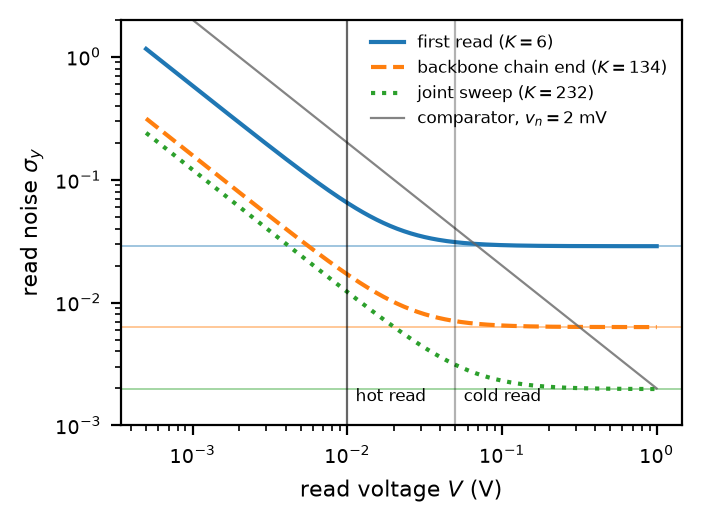
\includegraphics[width=\columnwidth]{figures/fig-noise.png}
\caption{Noise from the geometry model at settling-limited timing, including 5\,fF of comparator input capacitance. The first backbone read has six active label spaces; later pools are larger. Horizontal lines show flicker floors. The $v_n=2$\,mV comparator term exceeds device noise at the 10\,mV hot-read voltage.}
\label{fig:noise}
\end{figure}

\subsection{Readout assumptions}\label{app:readout}
The nominal readout uses a continuous-time comparator at 200\,nA and a lane buffer at 100\,nA, both at 0.8\,V for 62.5\,ns. These contribute 10 and 5\,fJ. No separate decision energy is added.

A falling reference approximates the emulator's single noise sample only if it crosses the comparator's $\pm3v_n$ band within one noise correlation time. The required slope is at least $6v_n\,2\pi B$. At $v_n=2$\,mV and bandwidth $B=500$\,MHz, this is about 38\,mV/ns, or a 20\,mV sweep in about 0.5\,ns.

Lower noise requires more bias energy. Using preamplifier noise $4\kB T\gamma B/g_m$ and $g_m=I/(nV_T)$ gives
\begin{equation}
E_{\mathrm{comp}}=
\frac{4\kB T\gamma\,nV_TV_{dd}(B t_r)}{v_n^2},
\end{equation}
where $t_r$ is readout duration. With $\gamma=1$, $nV_T=35$\,mV, and illustrative $Bt_r=3$, the estimates are 0.35\,fJ at 2\,mV, 1.4\,fJ at 1\,mV, 15\,fJ at 300\,$\mu$V, and 139\,fJ at 100\,$\mu$V. But 500\,MHz over 62.5\,ns gives $Bt_r=31.25$, increasing each by a factor of 10.4. These examples do not establish that the nominal budget meets both hot timing and cold noise requirements.

Alternative readouts also change the noise process. A five-strobe clocked search costs an estimated 55\,fJ per lane read including the buffer, and a 16-strobe ramp costs 165\,fJ. Both expose a decision to repeated noise samples. A pairwise tournament costs about 14\,fJ per lane on this census, but compares lane differences rather than independently perturbed lane scores. A 1\,$\mu$A continuous-time comparator costs 55\,fJ including the buffer and provides lower noise. None of these alternatives has been validated as an implementation of Eq.~\eqref{eq:draw}.

\subsection{Selection alternatives and omitted terms}
Grounding the nominal crossbar's unselected node-side lines isolates the selected signal but reduces its gain to about 0.31. Restoring the hot-read amplitude requires approximately 32.5\,mV and raises estimated image energy to 3.0\,nJ. Tracking those lines with a replica of the output voltage also gives an isolated read, but its approximately 3.0\,nJ estimate excludes the required replica buffer. The selector-column alternatives in Sec.~\ref{sec:energy} remove the node-side multiplexer and charge one select line per assertion. They require more select lines and leakage paths, with rails still pulsed per read.

The omitted rail-charging estimate is $5\times10^{-12}$\,J per image, about 0.3\% of the nominal total. An illustrative off-gate leakage calculation with 10\,ns pulses gives $2.5\times10^{-13}$\,J. Holding rails active for an assumed 30\,$\mu$s image would instead give $1.6\times10^{-10}$\,J; that assumed duration is not a timing bound.

Kickback is not established as negligible. An illustrative 0.5\,fC input charge moves a 131\,fF node by about 4\,mV, but a 12\,fF first-read node by about 42\,mV. Static trimming cannot be assumed to cancel state-dependent kickback over these loads. The 50\,mV cold read is below the modeled 0.10\,V erase and 0.25\,V write thresholds, but threshold separation alone does not validate a complete circuit.

The energy calculation is implemented in the repository module \path{chill_zen/energy_geom.py}. The companion repository's \texttt{NUMBERS.md} maps reported values to saved evidence and scripts, including energy scenarios, selection alternatives, and readout options. These estimates exclude programming, die area, and external communication, as does the cited DTM inference comparison. They are not bounds on an eventual implementation.

\section*{Declarations}
\subsection*{Data and code availability}
The companion repository is prepared for release at \url{https://github.com/knowm/CHILL-ZEN} under the MIT license. It contains the final experimental recipe, numerical evidence, and provenance of reported quantities. The lane emulator is available at \url{https://github.com/knowm/ktram-neural-core}. Evaluation imports the replication's feature extractor, distance code, and reference statistics; the companion repository records the commit, file checksums, and scoring harness without redistributing those assets. Intermediate fill-noise sweep logs were not retained, so those runs do not isolate the effect of training-fill noise.

\subsection*{Acknowledgments and AI assistance}
I thank the DTM authors for their detailed energy analysis and the replication authors for making their evaluation code available. AI tools assisted with running experiments, gathering data, drafting, and reviewing the manuscript. Review rounds included checks of the paper, code, logs, and cited DTM source. 

\subsection*{Competing interests}
The author is part of Knowm Inc., which has made and sold memristors and plans to commercialize technologies described here. The kT-bit, kT-RAM architecture, and technology stack are covered by granted U.S. patents \cite{nugent2015ktbitpatent,nugent2017ktrampatent,nugent2019stackpatent}. The portfolio is listed at \url{https://knowm.ai/ip/}.

\bibliography{refs}
\end{document}
